% ********** Appendix 1 **********

\graphicspath{{appendix/images/}}

\chapter{Principal Nested Spheres}
\label{sec:apendixCPNS}

PNS (Principal Nested Spheres) is an extension of PCA proposed to analyze data that lives on spherical manifolds. 
Examples of such data are directions like the spokes in s-reps (see Section \ref{sec:quasiMedial}).
Similarly to principal directions in PCA, PNS finds principal arcs through the data and gives a mechanism 
for dimension reduction. 
The term principal arc is defined by \cite{jung2011principal}.
%Instead of straight lines, PNS uses arcs.

This appendix is an overview of PNS, highlighting the construction of the Nested Spheres
and decomposition onto principal arcs. For details on the approach see \cite{jung_analysis_2012}.

%\begin{definition}
 %Given two points on the sphere, an \textbf{arc} is the shortest path or the segment of a circle that joins both points. 
%\end{definition}

PNS gives a more suited description of the data when major variations can be best described by potential arcs that are either 
small circles or great circles. 
This is in contrast to PGA (principal geodesic analysis),
which describes data variations using geodesics \cite{fletcher2004principal}, \cite{huckemann2010rejoinder}.

PNS decomposes the data space so that the major one-dimensional variation becomes linearly represented. 
For a unit \textit{d-sphere} $S^d$, which is the set of unit vectors in $R^{d+1}$. The analysis gives a 
decomposition of $S^d$ that captures the variation in a lower dimensional subsphere.
The subspheres are small spheres or great spheres depending on the type of analysis, \textit{i.e.}, by small circles or great circles. 
The type of analysis can be set by default or selected automatically with a hypothesis 
test that decides which type of subsphere to use. 

The sequential decomposition provides the best k-dimensional approximation $\varPsi_k$ of the data for
each $k = \{0, 1, . . . , d - 1\}$. The sphere $\varPsi_k$ is called the k-dimensional principal nested sphere and
is a submanifold of the higher dimensional principal nested spheres. The sequence of principal
nested spheres is
\begin{equation}
 \varPsi_0 \subset \varPsi_1 \subset ... \subset \varPsi_{d-1} \subset S^d.
 \label{equ:sequenceNestedSpheres}
\end{equation}

The procedure of fitting principal nested spheres involves iterative reduction of the data 
dimension.
The following section explains how to analyze the data using PNS.

\section{Computing PNS}

\subsection{Arc distance}

Equation \ref{equ:geodesic} shows the arc distance function between two points $x$ and $y$. The solution is unique unless
the points are antipodal, \textit{i.e.}, $x^Ty = -1$.
\begin{equation}
 \rho_d(x, y) = cos^{-1}(x^Ty)
 \label{equ:geodesic}
\end{equation}

\subsection{Subsphere}

Equation \ref{equ:subsphere} shows the definition
of a subsphere $A_{d-1}$ of $S^d$, 
defined by an axis $v \in S^d$ and a distance $r \in (0, \pi/2]$.

\begin{equation}
 A_{d-1}(v, r) = \{x \in S^d :  \rho_d(v, x) = r \}
 \label{equ:subsphere}
\end{equation}

The subsphere $A_{d-1}$ is an intersection of $S^d \subset R^{d+1}$
with a $d$-dimensional hyperplane such that $\{x \in R^{d+1}: v^Tx - cos(r) = 0\}$.

\subsection{Rotation to the north pole}

\begin{figure} 
 \centering 
 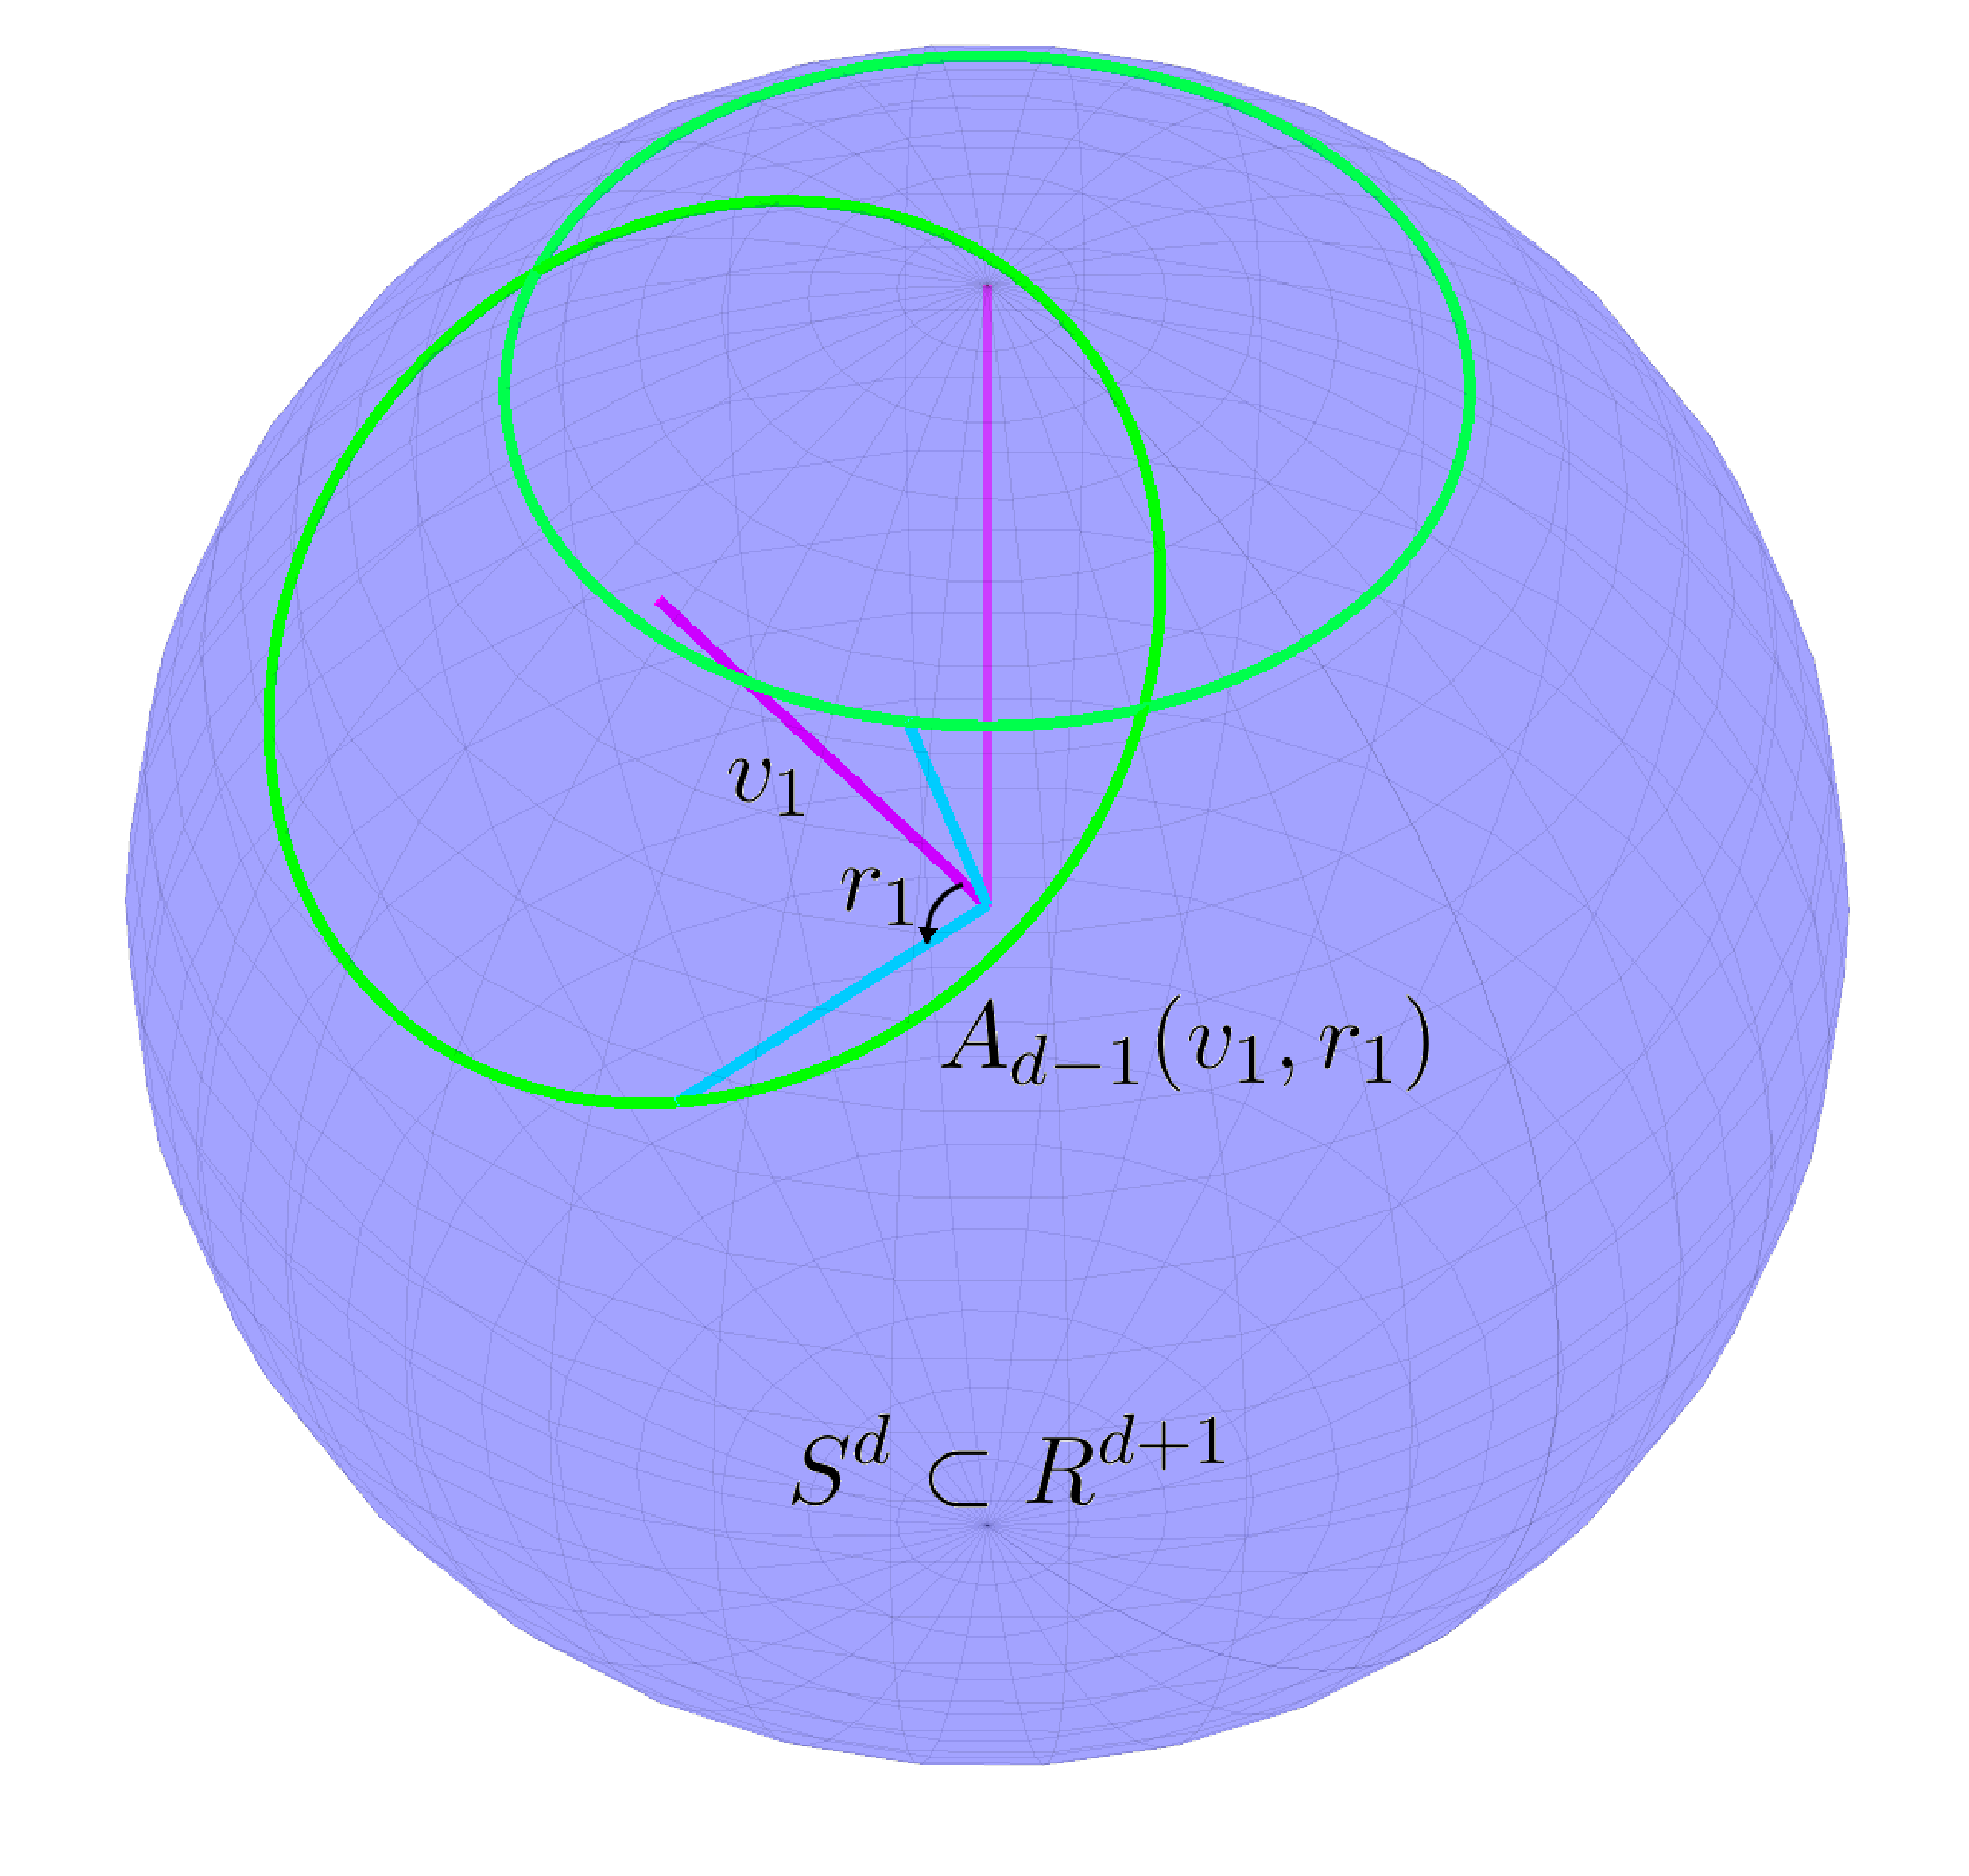
\epsfig{file = bestFitRotation.eps, width = 5cm}
 \caption{Rotation of the sub-sphere $A_{d-1}$ to the northpole.}
 \label{fig:rotateNorth}  
\end{figure}

Suppose that $a$ and $b$ are unit vectors in $R^m$, the rotation matrix $\Omega(a, b)$
moves $a$ to $b$ along a minimal path on the unit sphere.
\cite{amaral2007pivotal} defined a rotation matrix as
\begin{equation}
   \begin{array}{r}
      A = ac^T - ca^T\\
      c = {b - a(a^T b)}/||b - a(a^T b)||\\
      \theta = \rho_d(a, b)\\
      \Omega(a, b) = I_d + sin(\theta)A + {cos(\theta) - 1}(aa^T + cc^T).
    \end{array}
 \label{equ:rotateNorth}
\end{equation}

\subsection{Transformation of subsphere}

\begin{equation}
 \begin{array}{r}
 f_k(x) = \frac{1}{sin(r_k)} R^{-}(v_k)x, x \in A_{d-k} \\
 f_k^{-1}(x^\dagger) = R^T(v_k) \left [ \begin{array}{c}
                                        sin(r_k) \cdot x^\dagger \\
                                        cos(r_k) \end{array} \right ],
                       x^\dagger \in S^{d-k}
 \end{array}
 \label{equ:subFunction}
\end{equation}

Equation \ref{equ:subFunction} shows the function $f$ that enables going from a sphere dimension $S^d$ to a sub-sphere $S^{d-1}$
and the corresponding inverse, where $x \in A_{d-1}$, $x^\dagger \in S^{d-k}$.
Matrix $R$, rotates the data to the north pole.
$R = \Omega(v_k, e_k)$, where $e_k$ is the north pole, \textit{i.e.}, $e_k = (0,...,0,1)^T$.
$R^{-}$ is the $m \times m+1$ matrix consisting of the first $m$ rows of $R$.

\subsection{Best fitting subsphere}

\begin{figure} 
 \centering 
 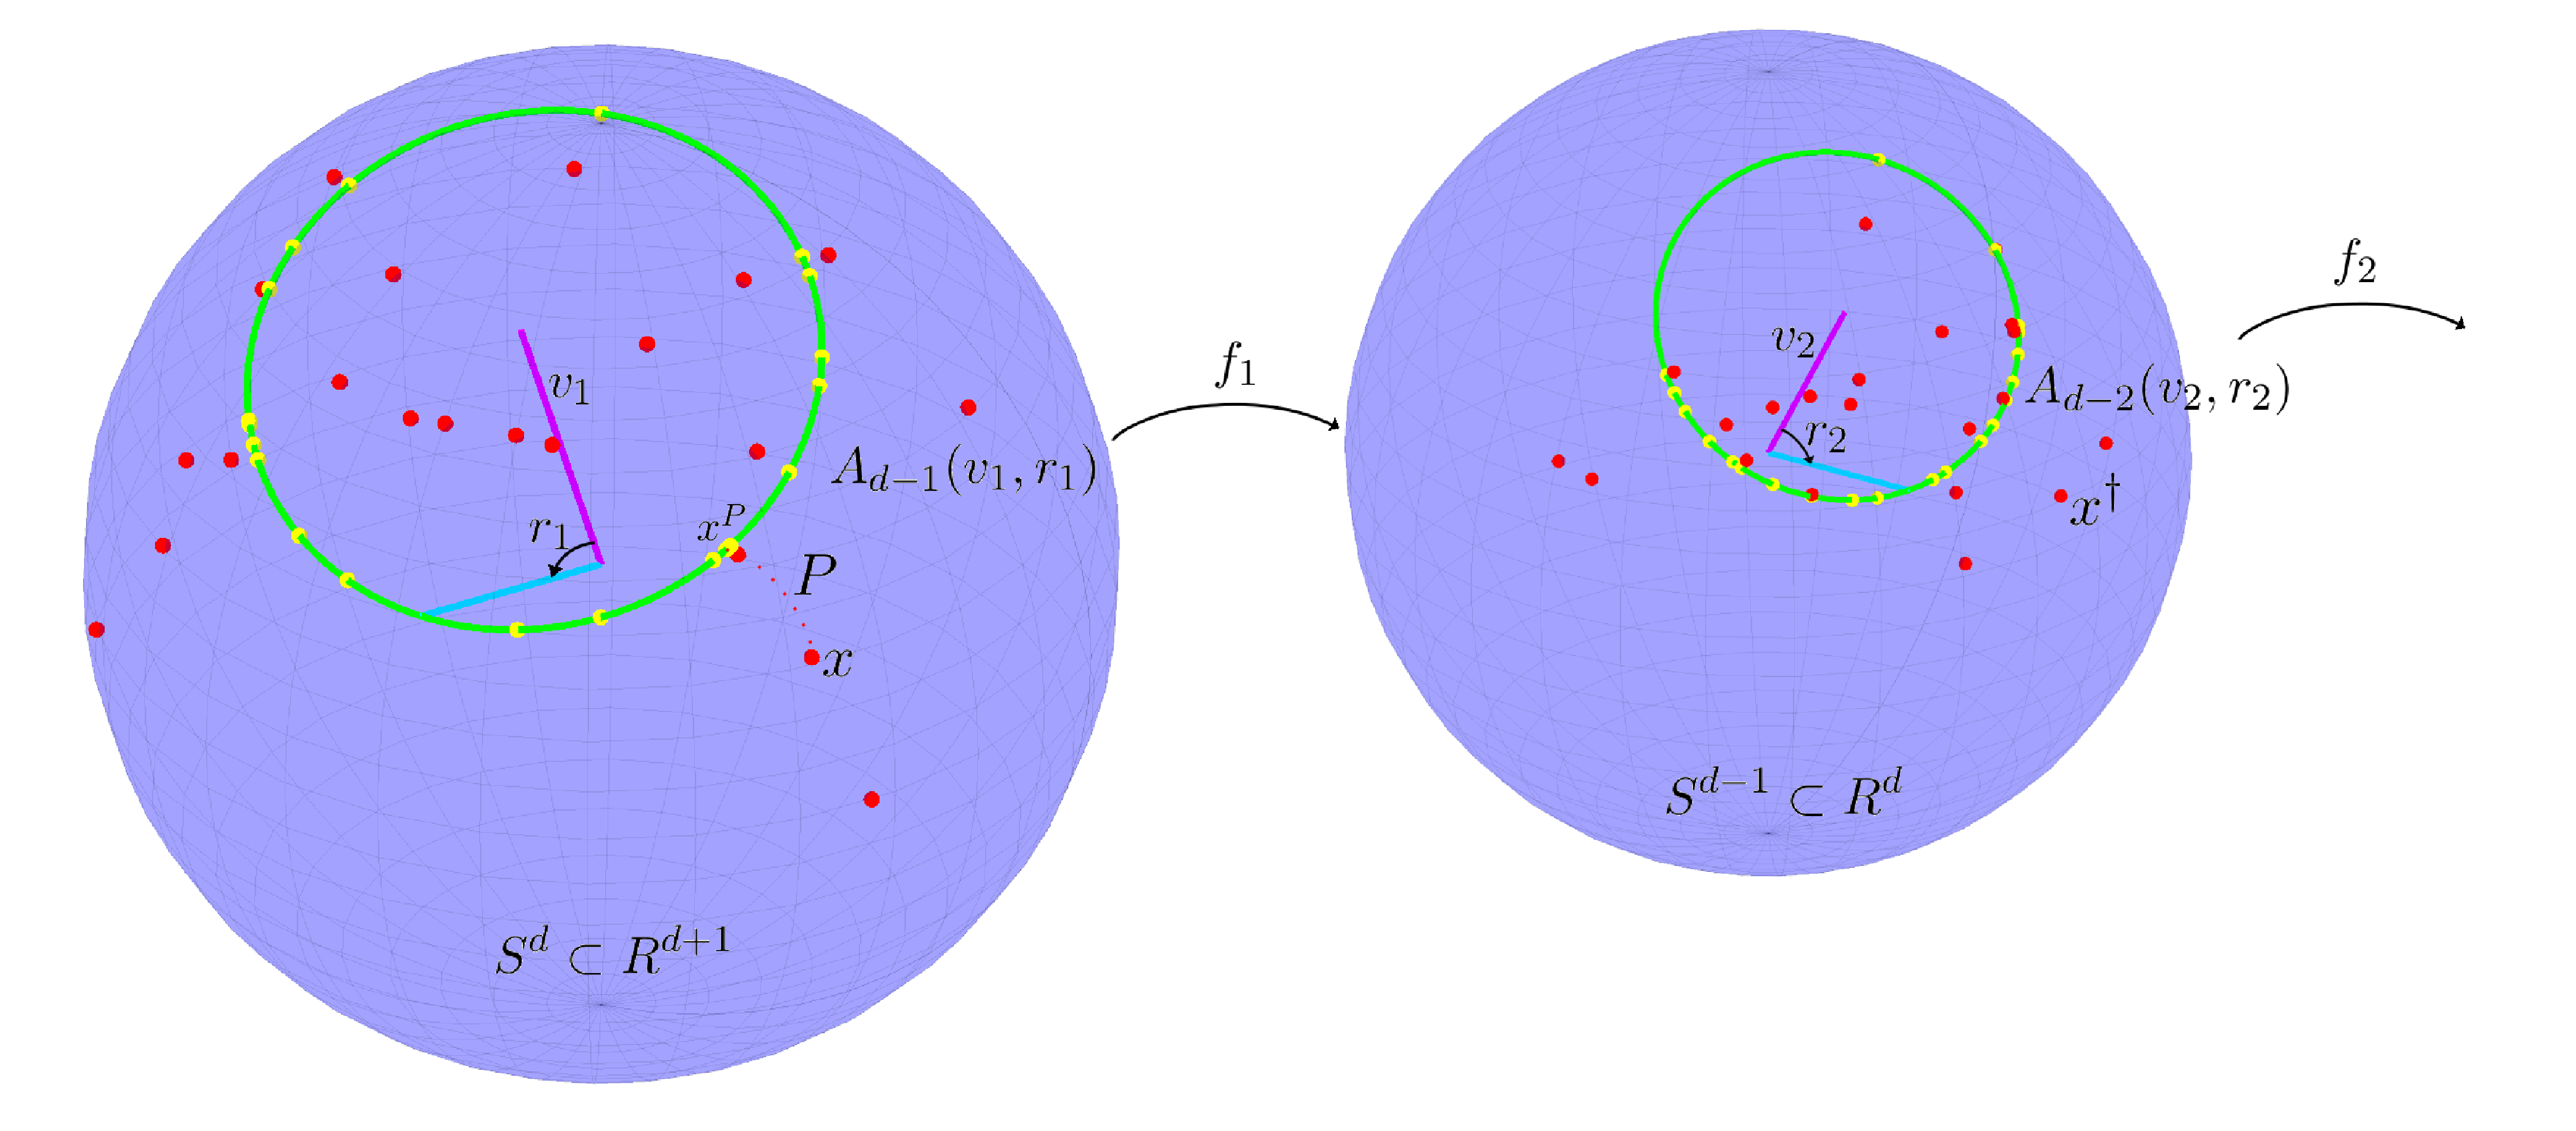
\epsfig{file = bestFittinSpherek.eps, width = 14cm} 
 \caption[Best fitting sphere and projection to sub-sphere]{The data points $x$ are shown in red, the best fitting sub-sphere to the data is shown in green $A_{d-1}(v_1, r_1)$, the vector $v_1$ is shown in magenta,
          the projected data points $x^P = P(x)$ in yellow on top of the best fitting circle. 
          Function $x^\dagger = f_1(x^P)$ takes the projected points on $A_{d-1}(v_1, r_1)$ to the sub-sphere $S^{d-1}$.}
 \label{fig:bestFittingSphere}  
\end{figure}

Let $x_1, ..., x_n$ be a sample in $S^d$, $d \geq 2$. The shortest distance 
from $x$ to a subshpere $A_{d-1}(v_1, r_1)$ of $S^d$ 
is the lenght of the minimal path that joins $x$ to $A_{d-1}$. 

The best fitting subsphere $\hat A_{d-1} = A_{d_1}(\hat v_1, \hat r_1)$ 
is found by minimizing the sum of squares of residuals of the data points to $\hat A_{d-1}$.
Equation \ref{equ:bestsubsphere} shows the procedure to find the best fitting subsphere.

\begin{equation}
 \hat A_{d-1}  = \operatorname*{Arg\,min}_{v_1, r_1} \sum_{i=1}^{n} \varepsilon_i ( v_1 , r_1 )^2 = \operatorname*{Arg\,min}_{v_1, r_1} \sum_{i=1}^{n} \big( \rho_d(x_i, v_1) - r_1 \big)^2
 \label{equ:bestsubsphere}
\end{equation}

Once the sub-sphere is found the points are projected to it, as shown in Equation \ref{equ:projectionSubSphere}.

\begin{equation}
 P\big( x, A_{d-1}(v, r) \big) = \frac{sin(r) x + sin\big(\rho_d(x, v) - r\big)v}{sin\big(\rho_d(x, v)\big)}
 \label{equ:projectionSubSphere}
\end{equation}

Let $x^P = P(x,\hat A_{d-1})$ be the projected point on the sub-sphere.
$x^P$ can be transformed from $\hat A_{d-1}$ to $S^{d-1}$ using the formula defined at \ref{equ:subFunction},
$x^\dagger = f(x^P)$ with $v_k = \hat v_1$ and $r_k = \hat r_1$.

Figure \ref{fig:bestFittingSphere} shows an example of finding the best fitting sub-sphere for the data points.

\subsection{Sequence of principal nested spheres}

The method finds the sequence of best fitting sub-spheres from 
the projected data points $\hat f \big ( P(x, \hat A_{d-k}) \big) \in S^{d-k} ( x \in S^{d-k+1})$. 
When a sub-sphere is fitted, the residuals defined by $\varepsilon_{i, d - k}$ are kept for later use as 
analogues of principal component scores.

The lowest best fitting sub-sphere $\hat A_1$ is a small circle isomorphic to $S^1$.
Since no further sphere or circle can be used to reduce the dimensionality, 
the Fr\'{e}chet mean is computed. 
Equation \ref{equ:frechetMean} defines the Fr\'{e}chet mean \cite{frechet1944integrale}, \cite{frechet1948elements}, \cite{karcher1977riemannian}, \cite{bhattacharya2003large}.

\begin{equation}
 \hat A_0 = \operatorname*{Arg\,min}_{x \in S^1} \sum_{i = 1}^n \rho_1(x, x_i^\dagger)^2
 \label{equ:frechetMean}
\end{equation}

The sequence of principal nested spheres in $S^d$ is $\{ \hat \varPsi_0, ..., \hat \varPsi_{d-1}\}$,
where $\hat \varPsi_{d - k}$ is defined as shown in Equation \ref{equ:principalNested}.
$\hat \varPsi_0$ is the principal nested spheres mean.

\begin{equation}
 \varPsi_{d - k} = \left\{ \begin{array}{ll}
                              \hat f_1^{-1} \circ ... \hat f_{k - 1}^{-1} &	(k = 2, ..., d), \\
                              \hat A_{d - 1}  & (k = 1) \end{array} \right.
 \label{equ:principalNested}
\end{equation}

Similarly,
the mean value $\hat A_0$ can be projected back to $S^d$ 
by recursively composing the inverse functions
as shown in Equation \ref{equ:principalNested}.
%If $\bar A_0^\dagger = A_0$ is the mean value at the lowest fitting sub-sphere, then 
%at $S^d$ is $\bar A_{d-k} = f_{d-k}^{-1}(f_{d-k+1}^{-1}(\hat A_{d-k+1}^\dagger))$.


\section{Residuals and principal arcs}

The signed residuals $\varepsilon_{i, d - k} (i = 1, ..., n)$ collected during the fitting process
are rescaled to make them commensurate. 
This is done by multiplying $\prod_{i = 1}^{k - 1} sin(\hat r_i)$ 
to the residuals as
\begin{equation}
 \Xi(d - k)_{1 \times n} = \prod_{i = 1}^{k - 1} sin(\hat r_i) (\varepsilon_{i, d - k}, ..., \varepsilon_{n, d - k}).
 \label{equ:commensurateResiduals}
\end{equation}
where $(\varepsilon_{i, d - k}, ..., \varepsilon_{n, d - k})$ is a row vector of residuals. 

The commensurate residuals are combined into a $d \times n$ matrix.
Each entry in $\Xi(k)$ lies in a subset of $E = [ \pi, \pi] \times [-\pi/2, \pi/2)^{d-1}$
and correspond to the sample's coordinates in terms of the principal nested sphere.

\begin{equation}
  \hat X_{PNS} = \left [ \begin{array}{c}
                          \Xi(0) \\
                          \Xi(1) \\
                          . \\
                          . \\
                          . \\
                          \Xi(d-1) \\
                         \end{array} \right ]
 \label{equ:principalResiduals}
\end{equation}

To compute the principal arcs (analogues to principal directions), 
each point in $S^d$ can be mapped to $E$ using the projection \ref{equ:projectionSubSphere} and rescaling.
Leading to a mapping $h: S^d \rightarrow E$.
The $k$th principal arc $\gamma_k$ coincides with direction $e_k$ and is parameterized
by $\gamma_k(t) = h(te_k)$, where $e_k$ is a vector of zeros with 1 at the $k$th position. 

The matrix $\hat X_{PNS}$ can be used to visualize the structure of the data.
Further analysis can be done on $\hat X_{PNS}$ using conventional multivariate statistics based on Euclidean geometry such as PCA.

% ********** End of appendix **********
